\subsection{基本作图}\label{subsec:czjh1-3-11}

先介绍几种最简单最常用的尺规作图,通常称为\zhongdian{基本作图}。
其他较复杂的作图,都是由基本作图组成的。

\begingroup
\ctexset {
  subsubsection = {
    number=\Roman{subsubsection},
    aftername={. },
  },
}

\begin{enhancedline}
\subsubsection{作一个角等于已知角。}

已知:$\angle AOB$ (图 \ref{fig:czjh1-3-41})。

求作:$\angle A'O'B'$,使 $\angle A'O'B' = \angle AOB$。

\zuofa 1. 作射线 $O'A'$。

2. 以点 $O$ 为圆心,以任意长为半径作弧,交 $OA$ 于 $C$, 交 $OB$ 于 $D$。

3. 以点 $O'$ 为圆心,以 $OC$ 长为半径作弧,交 $O'A'$ 于 $C'$。

4. 以点 $C'$ 为圆心,以 $CD$ 长为半径作弧,交前弧于 $D'$。

\begin{wrapfigure}[6]{r}{7cm}
    \centering
    % 严格按照作图的步骤绘制
\begin{tikzpicture}
    \tkzDefPoints{0/0/O, 2/0/A}
    \tkzDefPoint(40:2){B}
    \tkzDrawSegments(O,A  O,B)
    \tkzLabelPoints[left](O)
    \tkzLabelPoints[right](A)
    \tkzLabelPoints[above right](B)

    % 1
    \tkzDefPoints{3.5/0/O', 5.5/0/A'}
    \tkzDrawSegment(O',A')
    \tkzLabelPoints[left](O')
    \tkzLabelPoints[right](A')

    % 2
    \pgfmathsetmacro{\r}{1.5}
    \tkzInterLC[R,near](A,O)(O,\r)  \tkzGetFirstPoint{C}
    \tkzInterLC[R,near](B,O)(O,\r)  \tkzGetFirstPoint{D}
    \tkzDrawArc[delta=10](O,C)(D)
    \tkzLabelPoints[below left](C)
    \tkzLabelPoints[left](D)
    \tkzDrawSegment[dashed](C,D)

    % 3
    \tkzDrawArc[R](O',\r)(-10,50)
    \tkzInterLC[R,near](A',O')(O',\r)  \tkzGetFirstPoint{C'}
    \tkzLabelPoints[below left](C')

    % 4
    \tkzCalcLength(C,D)  \tkzGetLength{cd}
    \tkzDrawArc[R](C',\cd)(90,125)
    \tkzInterCC[R](O',\r)(C',\cd)  \tkzGetFirstPoint{D'}
    \tkzLabelPoints[left=0.5em](D')
    \tkzDrawSegment[dashed](C',D')

    % 5
    \tkzDefPointOnLine[pos=1.4](O',D')  \tkzGetPoint{B'}
    \tkzDrawSegment(O',B')
    \tkzLabelPoints[above right](B')
\end{tikzpicture}


    \caption{}\label{fig:czjh1-3-41}
\end{wrapfigure}

5. 经过点 $D'$ 作射线 $O'B'$。

$\angle A'O'B'$ 就是所求的角。

\zhengming 连结 $CD$、$C'D'$。 由作法可知

\qquad $\triangle C'O'D' \quandeng \triangle COD$ ($SSS$),

$\therefore$ \quad $\angle C'O'D' = \angle COD$(全等三角形对应角相等),

即 \quad $\angle A'O'B' = \angle AOB$。


\subsubsection{平分已知角。}

已知:$\angle AOB$ (图 \ref{fig:czjh1-3-42})。

求作:射线 $OC$, 使 $\angle AOC = \angle BOC$。

\zuofa 1. 在 $OA$ 和 $OB$ 上,分别截取 $OD$、$OE$,使 $OD = OE$。

2. 分别以 $D$、$E$ 为圆心, 大于 $\exdfrac{1}{2} DE$ 的长为半径作弧, 在 $\angle AOB$ 内, 两弧交于点 $C$。

\begin{wrapfigure}[6]{r}{6cm}
  \centering
  % 严格按照作图的步骤绘制
\begin{tikzpicture}
    \tkzDefPoints{0/0/O, 3/0/A}
    \tkzDefPoint(45:3){B}
    \tkzDrawSegments(O,A  O,B)
    \tkzLabelPoints[below](O,A)
    \tkzLabelPoints[above right](B)

    % 1
    \pgfmathsetmacro{\r}{1.5}
    \tkzInterLC[R,near](A,O)(O,\r)  \tkzGetFirstPoint{D}
    \tkzInterLC[R,near](B,O)(O,\r)  \tkzGetFirstPoint{E}
    \tkzDrawArc[delta=10](O,D)(E)
    \tkzLabelPoints[below left](D)
    \tkzLabelPoints[left=0.5em](E)

    % 2
    \tkzCalcLength(D,E)  \tkzGetLength{de}
    \tkzInterCC[R](D,\de)(E,\de)  \tkzGetSecondPoint{C}
    % \tkzDrawArc[R](D,\de)(30,60)
    % \tkzDrawArc[R](E,\de)(-20,10)
    \tkzCompasss(D,C  E,C)
    \tkzDrawSegments[dashed](D,C  E,C)
    \tkzLabelPoints[above right,yshift=0.3em](C)

    % 3
    \tkzDrawLine[add=0 and 0.3](O,C)
\end{tikzpicture}


  \caption{}\label{fig:czjh1-3-42}
\end{wrapfigure}

3. 作射线 $OC$。

$OC$ 就是所求的射线。

\zhengming 连结 $CD$、$CE$,由作法可知

\qquad $\triangle ODC \quandeng \triangle OEC$($SSS$),

$\therefore$ \quad $\angle COD = \angle COE$ (全等三角形对应角相等),

即 \quad $\angle AOC = \angle BOC$。


\subsubsection{经过一点作已知直线的垂线。}

(1) 经过已知直线上的一点作这条直线的垂线。

已知:直线 $AB$ 和 $AB$ 上一点 $C$ ( 图 \ref{fig:czjh1-3-43}) 。

求作: $AB$ 的垂线, 使它经过点 $C$。

\zuofa 作平角 $ACB$ 的平分线 $CF$。

直线 $CF$ 就是所求的垂线。

证明:由作法可知,

\qquad $\angle ACF = \angle BCF = \exdfrac{1}{2} \angle ACB$。

$\because$ \quad $\angle ACB = 180^\circ$(平角的定义),

$\therefore$ \quad $\angle ACF = 90^\circ$ (等量代换),

即 \quad $CF$ 是 $AB$ 的垂线。

\begin{figure}[htbp]
  \centering
  \begin{minipage}[b]{7cm}
      \centering
      % 严格按照作图的步骤绘制
\begin{tikzpicture}
    \tkzDefPoints{0/0/A, 4/0/B}
    \tkzDefPointOnLine[pos=0.45](A,B)  \tkzGetPoint{C}
    \tkzDrawSegments(A,B)
    \tkzLabelPoints[below](A,B)
    \tkzLabelPoints[below left](C)

    % 1
    \pgfmathsetmacro{\r}{1.3}
    \tkzInterLC[R,near](A,C)(C,\r)  \tkzGetFirstPoint{D}
    \tkzInterLC[R,near](B,C)(C,\r)  \tkzGetFirstPoint{E}
    \tkzCompasss[delta=8](C,D  C,E)
    \tkzLabelPoints[below=0.3em](D,E)

    % 2
    \tkzCalcLength(D,E)  \tkzGetLength{de}
    \pgfmathsetmacro{\r}{0.75*\de}
    \tkzInterCC[R](D,\r)(E,\r)  \tkzGetFirstPoint{F}
    \tkzCompasss(D,F  E,F)
    \tkzLabelPoints[above right,yshift=0.3em](F)

    % 3
    \tkzDrawLine[add=0.3 and 0.3](C,F)
\end{tikzpicture}

      \caption{}\label{fig:czjh1-3-43}
  \end{minipage}
  \qquad
  \begin{minipage}[b]{7cm}
      \centering
      % 严格按照作图的步骤绘制
\begin{tikzpicture}
    \tkzDefPoints{0/0/A, 4/0/B, 2/1.5/C}
    \tkzDrawSegments(A,B)
    \tkzLabelPoints[below](A,B)
    \tkzDrawPoint(C)
    \tkzLabelPoints[right](C)

    % 1
    \tkzDefPoints{1.5/-0.5/K}
    \tkzDrawPoint(K)
    \tkzLabelPoints[below](K)

    % 2
    \tkzCalcLength(C,K)  \tkzGetLength{ck}
    \pgfmathsetmacro{\r}{\ck}
    \tkzInterLC[R](A,B)(C,\r)  \tkzGetPoints{D}{E}
    \tkzLabelPoints[above](D,E)
    \tkzDrawArc[delta=10](C,D)(E)

    % 3
    \tkzCalcLength(D,E)  \tkzGetLength{de}
    \pgfmathsetmacro{\r}{0.75*\de}
    \tkzInterCC[R](D,\r)(E,\r)  \tkzGetSecondPoint{F}
    \tkzDrawPoint(F)
    \tkzCompasss(D,F  E,F)
    \tkzLabelPoints[right=0.3em](F)

    % 4
    \tkzDrawLine[add=0.2 and 0.2](C,F)
\end{tikzpicture}


      \caption{}\label{fig:czjh1-3-44}
  \end{minipage}
\end{figure}

(2) 经过已知直线外一点作这条直线的垂线。

已知: 直线 $AB$ 和 $AB$ 外一点 $C$ (图 \ref{fig:czjh1-3-44})。

求作: $AB$ 的垂线, 使它经过点 $C$。

\zuofa 1. 任意取一点 $K$, 使 $K$ 和 $C$ 在 $AB$ 的两旁。

2. 以 $C$ 为圆心, $CK$ 长为半径作弧,交 $AB$ 于点 $D$ 和 $E$。

3. 分别以 $D$ 和 $E$ 为圆心,大于 $\exdfrac{1}{2} DE$ 的长为半径作弧,两弧交于点 $F$。

4. 作直线 $CF$。

直线 $CF$ 就是所求的垂线。

证明略。


\subsubsection{作线段的垂直平分线。}

\begin{wrapfigure}[8]{r}{6cm}
  \centering
  % 严格按照作图的步骤绘制
\begin{tikzpicture}
    \tkzDefPoints{0/0/A, 4/0/B}
    \tkzDrawSegments[xianduan={below=0pt}](A,B)
    \tkzLabelPoints(A,B)

    % 1
    \tkzCalcLength(A,B)  \tkzGetLength{ab}
    \pgfmathsetmacro{\r}{0.6*\ab}
    \tkzInterCC[R](A,\r)(B,\r)  \tkzGetPoints{C}{D}
    \tkzCompasss(A,C  B,C  A,D  B,D)
    \tkzLabelPoints[right](C,D)

    % 2
    \tkzDrawLine[add=0.2 and 0.2](C,D)
\end{tikzpicture}


  \caption{}\label{fig:czjh1-3-45}
\end{wrapfigure}


已知: 线段 $AB$ (图 \ref{fig:czjh1-3-45})。

求作:线段 $AB$ 的垂直平分线。

\zuofa 1. 分别以点 $A$ 和 $B$ 为圆心,大于 $\exdfrac{1}{2} AB$ 的长为半径作弧,两弧和交于点 $C$ 和 $D$。

2. 作直线 $CD$。

直线 $CD$ 就是线段 $AB$ 的垂直平分线。

证明略。

因为直线 $CD$ 与线段 $AB$ 的交点,就是 $AB$ 的中点,所以我们也用这种方法平分已知线段或作线段的中点。


\subsubsection{经过已知直线外的一点作这条直线的平行线。}

\begin{wrapfigure}[6]{r}{6cm}
  \centering
  \begin{tikzpicture}
    \tkzDefPoints{0/0/A, 4/0/B, 2.5/1.5/M}
    \tkzDrawSegment(A,B)
    \tkzLabelPoints[left](A)
    \tkzLabelPoints[right](B)
    \tkzLabelPoints[above, xshift=-0.3em](M)

    % 1
    \tkzDefPointOnLine[pos=0.3](A,B)  \tkzGetPoint{N}
    \tkzDefPointOnLine[pos=1.7](N,M)  \tkzGetPoint{P}
    \tkzLabelPoints[below, xshift=0.3em](N)
    \tkzLabelPoints[left](P)
    \tkzDrawLine[add=0 and 0.4](P,N)

    % 2
    \tkzDefLine[parallel=through M,normed](A,B)  \tkzGetPoint{x}
    \tkzDefPointOnLine[pos=1.5](M,x)  \tkzGetPoint{D}
    \tkzDefPointOnLine[pos=-2.3](M,x)  \tkzGetPoint{C}
    \tkzDrawSegment(C,D)
    \tkzLabelPoints[left](C)
    \tkzLabelPoints[right](D)
    \tkzMarkAngle[size=0.5](B,N,M)
    \tkzMarkAngle[size=0.5](D,M,P)
\end{tikzpicture}


  \caption{}\label{fig:czjh1-3-46}
\end{wrapfigure}


已知: 直线 $AB$ 和 $AB$ 外一点 $M$ (图 \ref{fig:czjh1-3-46})。

求作: 直线 $CD \pingxing AB$, 且 $CD$ 经过点 $M$。

\zuofa 1. 过点 $M$ 作直线 $MN$, 交直线 $AB$ 于 $N$。

2. 过点 $M$ 作直线 $CD$, 使同位角 $\angle PMD = \angle MNB$。

直线 $CD$ 就是所求的平行线。

\zhengming 由作法可知 $\angle PMD = \angle MNB$,

$\therefore$ \quad $CD \pingxing AB$ (同位角相等,两直线平行)。

\end{enhancedline}
\endgroup

\begin{lianxi}

用直尺和圆规作图,并口述作法:

\xiaoti{作一个角等于 $45^\circ$。}

\xiaoti{把已知线段 4 等分。}

\end{lianxi}



利用基本作图,可以进行其他作图。

\liti[0] 已知底边 $a$,底边上的高 $h$,求作等腰三角形。

已知:线段 $a$、$h$(图 \ref{fig:czjh1-3-47})。

\begin{figure}[htbp]
  \centering
  \begin{tikzpicture}
    \pgfmathsetmacro{\a}{2.5}
    \pgfmathsetmacro{\h}{4}

    \tkzDefPoints{0/0/h1, \h/0/h2, 0/0.8/a1, \a/0.8/a2}
    \tkzDrawSegments[xianduan={below=0pt}](h1,h2)
    \tkzLabelSegment[above](h1,h2){$h$}
    \tkzDrawSegments[xianduan={below=0pt}](a1,a2)
    \tkzLabelSegment[above](a1,a2){$a$}

    \begin{scope}[xshift=6cm]
        % 1
        \tkzDefPoints{0/0/B, \a/0/C}
        \tkzDrawSegment(B,C)
        \tkzLabelPoints[left](B)
        \tkzLabelPoints[right](C)

        % 2
        \tkzDefLine[mediator,normed](B,C)  \tkzGetPoints{m}{N}
        \tkzDefPointOnLine[pos=3](N,m)  \tkzGetPoint{M}
        \tkzInterLL(B,C)(M,N)  \tkzGetPoint{D}
        \tkzDrawSegment(M,N)
        \tkzMarkRightAngle(M,D,B)
        \tkzLabelPoints[right](M,N)
        \tkzLabelPoints[above right](D)

        % 3
        \tkzInterLC[R,near](M,N)(D,\h)  \tkzGetFirstPoint{A}
        \tkzLabelPoints[left](A)

        % 4
        \tkzDrawSegments(A,B  A,C)
    \end{scope}
\end{tikzpicture}


  \caption{}\label{fig:czjh1-3-47}
\end{figure}

求作: $\triangle ABC$, 使 $AB = AC$, 且 $BC = a$, 高 $AD = h$。

\zuofa 1. 作线段 $BC = a$。

2. 作线段 $BC$ 的垂直平分线 $MN$,$MN$ 与 $BC$ 交于点 $D$。

3. 在 $MN$ 上截取 $DA$,使 $DA = h$。

4. 连结 $AB$、$AC$。

$\triangle ABC$ 为所求的等腰三角形。

\zhengming 由作图可知, $\triangle ABD \quandeng \triangle ACD$ ($SAS$)。

$\therefore$  \quad $AB = AC$ (全等三角形对应边相等)。

又 $\because$ \quad $BC = a$, $AD \perp BC$, $AD = h$ (作图),

所以 $\triangle ABC$ 是所求的等腰三角形。

一般的几何作图题,应有下面几个步骤:已知、求作、作法、证明。
比较复杂的题,在作图之前可先作分析。
目前,我们只要求写出已知、求作、作法三个步骤。

\begin{lianxi}

作一个直角三角形,使它的两条直角边分别等于线段 $a$、$b$。

\begin{figure}[htbp]
  \centering
  \begin{tikzpicture}
    \tkzDefPoints{0/1/A,  4/1/B}
    \tkzDefPoints{0/0/C,  3/0/D}

    \tkzDrawSegments[xianduan={below=0pt}](A,B)
    \tkzDrawSegments[xianduan={below=0pt}](C,D)
    \tkzLabelSegment[above](A,B){$a$}
    \tkzLabelSegment[above](C,D){$b$}
\end{tikzpicture}

\end{figure}

\end{lianxi}

